%http://www.slideshare.net/boricles/linguistic-resources-enhanced-with-geospatial-information
In this section we present the specialisation of the Linked Data Life Cycle presented in \cite{Villazon_2011} applied to linguistics resources enhanced to geospatial information.

\subsection{Linguistics Resources}\label{sec:lr}

Our initial data source consisted of a spreadsheet containing GPS and lexical information for .... %STEVE FILL OUT 

\subsection{URI design}
All the resources in our dataset are defined using a URI\footnote{\url{http://tools.ietf.org/html/rfc3986}} (Uniform Resource Identifier). URIs have been designed with simplicity, stability and manageability in mind, following common guidelines for their effective use\footnote{\url{http://www.w3.org/TR/cooluris/}}, \footnote{\url{http://www.w3.org/Provider/Style/URI}}, \footnote{\url{http://www.w3.org/TR/chips/}}.

\subsubsection{Base URI structure}

\surl{http://linguistic.linkeddata.es/}

\subsubsection{Vocabulary elements}

\surl{http://linguistic.linkeddata.es/ontology/{property|class}}

For example

\surl{http://linguistic.linkeddata.es/ontology/officialName}

\subsubsection{Instances}

\surl{http://linguistic.linkeddata.es/dataset/resource/{r. type|r. name}}

For example

\surl{http://linguistic.linkeddata.es/mlode/Village/Sokoura}



\subsection{Modelling}
The development of the linguistics vocabulary, which covers the linguistic information stored in the resources described in section \ref{sec:lr}, 
has been performed following an iterative approach
based on the reuse of existing knowledge resources. In a nutshell we have reused the following vocabularies 
\begin{itemize}
	\item GOLD\footnote{\url{http://linguistic-ontology.org}}, an ontology for descriptive linguistics.
	\item WGS84 Geo Basic Vocabulary\footnote{\url{http://www.w3.org/2003/01/geo/}}, for representing the geospatial data	 
\end{itemize} 

Nevertheless, it was necessary to create some own terms.

\subsection{Generation}
RDF has been generated within three main phases. Next we describe each one of them.

\begin{enumerate}
	\item Importing the spreadsheet into MySQL database by using the MySQL importing tool.
	\item Defining a set of R2RML\footnote{R2RML is a standard RDB2RDF mapping language \url{http://www.w3.org/TR/r2rml/}} mappings among the MySQL database and RDF vocabulary elements.
	\item Executing the R2RML engine, morph\footnote{\url{https://github.com/boricles/morph}}, for generating the RDF instances from the MySQL database data by using the defined R2RML mappings.  
\end{enumerate}


\subsection{Publication}
The generated RDF is stored in Virtuoso\footnote{\url{http://virtuoso.openlinksw.com/}} open source version, which
integrates with Pubby\footnote{\url{http://www4.wiwiss.fu-berlin.de/pubby/}} to publish the results, making
them available for humans and computers.

\subsection{Exploitation}
The resultant dataset exposes the linguistics resources enhanced with geospatial information, allowing for queries that otherwise require a lot of time by just looking at the original files. 


By extending the queries presented previously, we have built an application\footnote{\url{http://geo.linkeddata.es/map4rdf-dogon/}} for showing each of the Dogon villages on the map by using the tool map4rdf\footnote{\url{https://github.com/boricles/linked-data-visualization-tools}} \cite{deLeon_2012}. Figure \ref{fig:map4rdf} shows the application.

\begin{figure*}[htb!p]
\centering
%\includegraphics[scale=0.45]{IMGS/detalle_bn.png}
%\includegraphics[width=0.70\textwidth]{IMGS/detalle.pdf}
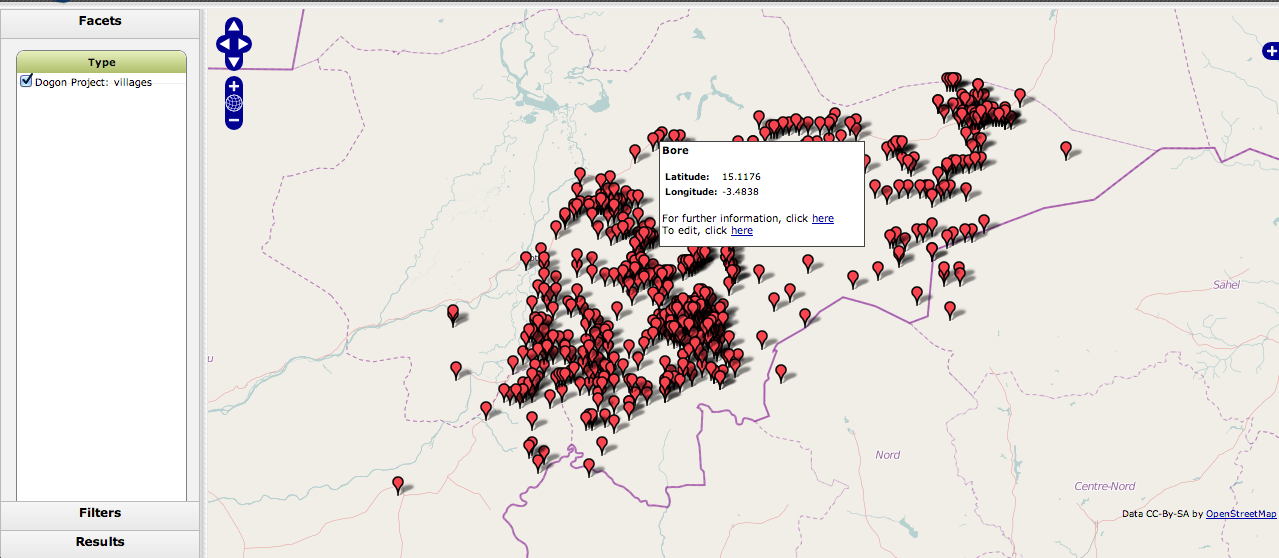
\includegraphics[width=0.99\textwidth]{img/map4rdf.png}
\caption{Visualization of the Dogon villages}
\label{fig:map4rdf}
\end{figure*}

%We then used the tool map4rdf\footnote{This can be accessed here: \url{http://code.google.com/p/map4rdf}} to map it upon a globe, with an online portal at: \url{http://oegdev.dia.fi.upm.es/projects/map4rdf} \cite{deLeon_2012} . At this stage, we have plotted each of the Dogon villages on the map. Each point also contains additional information about the language spoken in that village. The map is available here: \url{http://geo.linkeddata.es/map4rdf-dogon/#dashboard}


%I don't really know the details too much?